\documentclass[conference]{IEEEtran}
\IEEEoverridecommandlockouts
% The preceding line is only needed to identify funding in the first footnote. If that is unneeded, please comment it out.
\usepackage{cite}
\usepackage{amsmath,amssymb,amsfonts}
\usepackage{graphicx}
\usepackage{textcomp}
\usepackage{xcolor}
\usepackage{subfig}
\usepackage{algorithmic, algorithm}
\usepackage{hyperref}
\usepackage{hyperref} % makes cross-refs (biblio, figures, algos, ...) clickable
\def\BibTeX{{\rm B\kern-.05em{\sc i\kern-.025em b}\kern-.08em
    T\kern-.1667em\lower.7ex\hbox{E}\kern-.125emX}}

\newcommand{\logic}[1]{\color{red}\textbf{Logic/flow:}#1\color{black}}
\newcommand{\writing}[1]{\color{green}\textbf{Writing:}#1\color{black}}
\newcommand{\tristan}[1]{\color{orange}\textbf{From Tristan:}#1\color{black}}
\newcommand{\timothee}[1]{\color{blue}\textbf{From Timothée:}#1\color{black}}

\begin{document}

\title{Repartitioning large multi-dimensional arrays: a sequential algorithm and its implementation in Dask}

\author{\IEEEauthorblockN{Timoth\'ee Gu\'edon, Val\'erie Hayot-Sasson, Tristan Glatard \\
  \IEEEauthorblockA{
    Department of Computer Science and Software Engineering, Concordia University, Montreal, Canada
  }}
}

\maketitle

\begin{abstract}
Todo.
\end{abstract}

\begin{IEEEkeywords}
multidimensional, array, split, merge, resplit, IO, processing, Dask, Python
\end{IEEEkeywords}

%----------------------------------------
\section{Introduction}
%----------------------------------------
% big data challenges
With the improvement of acquisition methods and the growth in the amount of data
available in several scientific domains such as health
sciences~\cite{bigdata_health}~\cite{Amunts1472}, geology~\cite{big_data_geology}
and astrophysics~\cite{biguniverse}, new big data challenges have emerged related
to the processing of large amounts of data and ultra-high resolution
images. Big Brain, a human brain model providing microscopic data (20 micrometers) for
modeling and simulation~\cite{Amunts1472} is an example of ultra high resolution
images in the neuroscience field.

\subsection{Data storage on disk}
% use of chunking
Scientific data is often represented as multidimensional arrays stored in
chunks to facilitate processing and storage. Among other advantages, chunking
allows for efficient queries, flexibility in adding new
data~\cite{optimal_chuking}, parallel processing, and out-of-core
computations through block algorithms~\cite{matthew_rocklin-proc-scipy-2015}.

% explain storage order
Previous work focused on optimizing the data storage by looking for an optimal
chunk shape that would reduce the expected number of chunks to be retrieved by
any query~\cite{optimal_chuking} or by optimizing the ordering of the chunks
using space filling curves for example~\cite{optimal_chuking, openconnectomecluster}.
Instead, our approach is to leave the choice of the
data storage to the application as much as possible, as in~\cite{seqalgorithms}.
We therefore assume that the chunk shape and the data ordering in files are
arbitrary but known.

For the sake of clarity and without loss of generality,
 we assume in this study that files are written in row-major order (a.k.a
``C" order), where the fastest moving dimension in the file is the last
dimension in the array, and the slowest moving dimension in the file is the first
dimension in the array. For example a 3D array with dimensions $i$, $j$ and $k$
would be written on disk by writing the complete columns in the k dimension first
(see Figure~\ref{fig:seeks_and_rowmajor} (a)).
Our experiments use the HDF5~\cite{hdf5} file format as it is commonly used in the
scientific community and it is written in \texttt{C-order} by default.

\begin{figure*}[h]
  \centering
  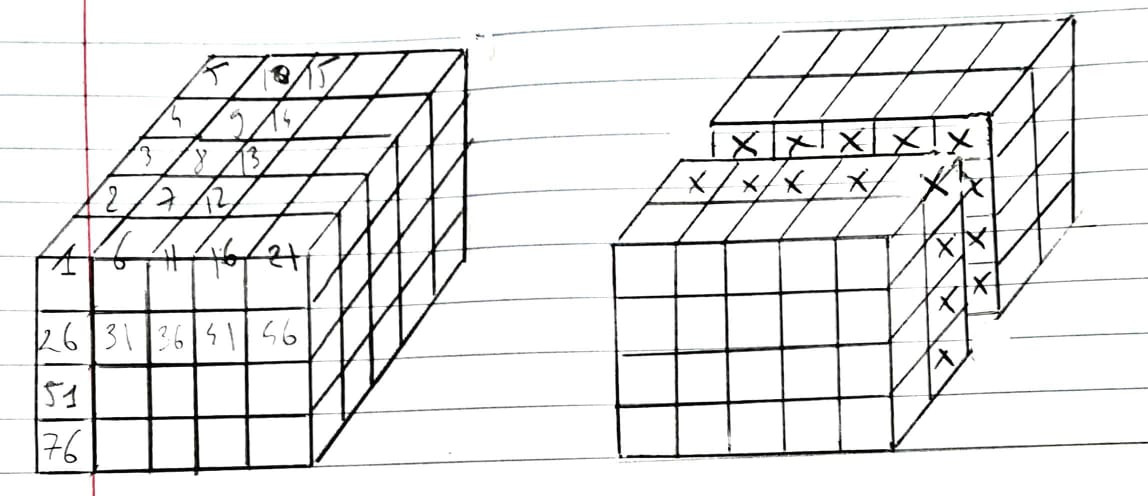
\includegraphics[scale=0.35]{./figures/new/seeks_and_rowmajor.jpeg}
  \caption{Illustration of the r\texttt{C-order} in files. The left subfigure
  shows how the data is written on disk, with each cube representing a voxel. The
  right subfigure shows how reading or writing only one part of a cuboid written
  in the \texttt{C-order} can produce seeks. Each cross represents a seek.}
  \label{fig:seeks_and_rowmajor}
\end{figure*}

\subsection{Multidimensional array chunking}

% need for tools to repartition
Using chunked multidimensional arrays requires tools to efficiently split,
merge, and ``resplit" or ``repartition" data files. Previous work in~\cite{seqalgorithms}
showed that naive algorithms to split an array into several chunks or merge
array chunks into one output file do not perform well due to millions of seeks
occurring on disk. The present study is focused on sequential algorithms for
repartitioning multidimensional arrays, letting the parallel and distributed
cases as future work, although they are relevant, too. To the best of our
knowledge, the repartition problem has not been extensively studied.

% why subarray extraction incurs seeks
Retrieving sub-arrays from an array stored on disk incurs seeks in two
situations: (1) when an array block is opened for reading or writing, and (2)
when the reading or writing process moves within the block to access a
contiguous piece of data. For a 3D cuboid of shape $C = (C_i, C_j, C_k)$ stored
in row-major order, each column of data in the k dimension is contiguously
stored. There are therefore $C_j \times C_i$ data columns that all require a
seek (see Figure~\ref{fig:seeks_and_rowmajor} (b)).
Although the seek time depends on various parameters such as the distance
in bytes between two data columns, we assume that all seeks incur the same time
overhead for the sake of simplicity. Therefore our problem will be to minimize
the number of seeks required to access data.

Not only extracting a subarray from a chunk incurs seeks on disk, but also
accessing any piece of data from a chunk results in loading the whole chunk in
memory. Chunking must therefore be used with care as it can be detrimental for
performance. The Python library \texttt{h5py} for manipulating HDF5 files
recommends a chunk size ``between 10 KiB and 1 MiB" and more for larger
datasets~\cite{collette_2014}. \texttt{dask}, a popular Python package, part of
the SciPy ecosystem, enabling parallel and out-of-core
computations~\cite{matthew_rocklin-proc-scipy-2015} also mentions the issues
relative to chunking and suggests a chunk size greater than 100 MB, although
remainding that the chunk shape selection is highly dependent on the
application~\cite{rocklin_bourbeau_2019}.

\subsection{Contributions}
This paper makes the following contributions:
\begin{itemize}
  \item The definition of the re-partition problem for multidimensional arrays
  \item The proposition of a sequential algorithm to efficiently
  re-partition multidimensional arrays
  \item An open implementation of this algorithm on Github
\end{itemize}

\section{Problem definition}
\subsection{The re-partition problem}
We focus on 3D arrays for simplicity. Consider a 3D array of shape $R =
(R_i, R_j, R_k)$, partitioned as input chunks of uniform shape $I = (I_i,
I_j, I_k)$ stored on disk. Our goal is to re-partition the input blocks into
output blocks of uniform but different shape $O = (O_i, O_j, O_k)$.
A re-partitioning algorithm reads the input blocks from disk, and writes the
output blocks to disk.

We present hereafter a general algorithm for the re-partition task.

A re-partioning algorithm (Algorithm~\ref{algo:generalrepartition}) takes a
list of input blocks \texttt{inBlocks} of shape $I$, a list of output block
definitions \texttt{outBlocks} of shape $O$ and the amount of memory \texttt{m}
available for the algorithm.
Subject to $m$, the algorithm first defines a list of buffers, the
\texttt{readBuffers}, to read from the input blocks (line 9).
These buffers have the same shape $B$.
Then, the algorithm computes another list of buffers, the \texttt{writeBuffers},
in which each buffer is a piece of data to be written at a time into an
output file (line 10).
In other words, the write buffers describe how each output file will be written.
All readBuffers have the same shape $B$. On the contrary, the writeBuffers can
have different shapes.
Finally, the main loop of the algorithm (line 12) loads one readBuffer at a
time (line 13), inserts it into a cache (line 14), and writes each writeBuffer
as soon as its data is available in cache (lines 15 to 18).

In this study, we express the quantity of memory used by an array as the
number of voxels it contains. It is equivalent to saying that the number of
bytes per voxel is 1. With $\alpha$ the number of bytes per voxel in the storage
device, $m$ is defined as $m/\alpha$.

For simplicity, we require that all buffers in \texttt{readBuffers} have
the same shape $B$. We define the cost function $\mathrm{seeks}$ as returning
the number of seeks incurred by the repartitioning algorithm.
The re-partitioning problem is therefore to find the best read and write buffers
lists in order to minimize $\mathrm{seeks}$ subject to $m$.
Solutions of this problem materialize as implementations of function
\texttt{getReadBuffers} and \texttt{getWriteBuffers} in
Algorithm~\ref{algo:generalrepartition}.

A lower bound on the number of seeks for the repartitioning problem is
$n_i + n_o$, with $n_i$ the number of input files and $n_o$ the number of output
files. Indeed, input and output files all have to be accessed at least once,
which requires a seek.

\begin{algorithm}
  \caption{General re-partitioning algorithm}
  \label{algo:generalrepartition}
  \begin{algorithmic}[1]
    \STATE \textbf{Inputs}
    \STATE inBlocks: input chunks stored in one dedicated file (or in one dataset of a HDF5 file).
    \STATE outBlocks: output chunks to be written, created as one empty file (/dataset of a HDF5 output file).
    \STATE $m$: memory available for one readBuffer or writeBuffer
    \STATE $I$: shape of one input chunk
    \STATE $O$: shape of one output chunk
    \STATE
    \STATE \textbf{Algorithm}
    \STATE B, readBuffers $\leftarrow$ getReadBuffers($I$,$O$,$m$)
    \STATE writeBuffers $\leftarrow$ getWriteBuffers($O$, $B$)
    \STATE initialize(cache)
    \FOR{readBuffer in readBuffers}
      \STATE bufferData $\leftarrow$ read(readBuffer, inBlocks)
      \STATE cache.insert(bufferData)
      \FOR{writeBuffer in writeBuffers}
        \IF{cache.isComplete(writeBuffer)}
          \STATE data = cache.pop(writeBuffer)
          \STATE write(writeBuffer, outBlocks)
        \ENDIF
      \ENDFOR
    \ENDFOR

  \end{algorithmic}
\end{algorithm}

\subsection{The multiple and clustered strategies}
Special cases of the re-partitioning problem occur when $I=R$ (``split'' problem)
or when $O=R$ (``merge'' problem). Two strategies were introduced
in~\cite{seqalgorithms} to address these problems: the ``multiple" and the
``clustered" strategies. In these strategies, every loaded buffer is directly written to the
destination output files.
The only difference between the multiple and the clustered strategies lies in
the selection of $B$.

In the split problem studied in~\cite{seqalgorithms} ($I=R$), a \texttt{naive}
strategy defines the read buffers as having the same shape than the output blocks
($B$=$O$). The read buffers are iteratively loaded from $R$ and entirely written
to the appropriate output block (represented by a writeBuffer of shape $O$, too).
The \texttt{clustered} strategy, however, loads as
many contiguous data blocks of shape $O$ as possible to fit in $m$.
$B$ is therefore a multiple of $O$.
Depending on the amount of main memory available, the data blocks may be loaded
individually, by entire block columns, or by entire block slabs.
Although this strategy allows to write each output block in one seek
(for opening the output file), the clustered strategy is limited by the fact
that it does not optimize the reading step.
In the case of the re-partition task, one can expect the clustered strategy to
perform poorly as
(1) it reads an output block no matter if it is split in a lot of different input blocks
and (2) even if it is stored in one input block the algorithm will do a lot of seeks in
case of a shape mismatch.
These limits are exacerbated in the re-partition task as there are many input and
output files.

The \texttt{multiple} strategy used for the split problem in~\cite{seqalgorithms}
aims at not doing any seek while reading \textit{and} writing;
Both the input and the output blocks are read/written contiguously. In
terms of Algorithm~\ref{algo:generalrepartition}, this means defining read buffers as
contiguous parts of the input array and write buffers as contiguous parts of
the output arrays. It is equivalent to extending the buffer in the inverse of
the storage order: $k \rightarrow j \rightarrow i$ in the case
of the \texttt{C-order}. The tradeoff lies in switching between files
at each buffer loading. In this case too, using this strategy for the re-partition task would
result in even more switches between input and output files which makes the limit
even more important.

To the best of our knowledge, no algorithm has been proposed for the
repartitioning task.

\subsection{Baseline solution}

Our baseline algorithm for the repartitioning problem loads one input block
at a time, that is, $B$=$I$ in Algorithm~\ref{algo:generalrepartition},
and directly writes it to the appropriate output blocks.
The write buffers are therefore defined by the intersections between the input
and output blocks.
For the baseline algorithm, we assume that one input block fits in memory ($m \geq I_iI_jI_k$).
As in Algorithm~\ref{algo:generalrepartition}, each buffer is only loaded once.

The number of seeks $s$ induced by this baseline algorithm is the
sum of the number of seeks done for each buffer, that is, the sum of:
\begin{itemize}
  \item the number of input blocks (1 seek per read buffer)
  \item the number of output blocks openings
  \item the number of seeks done by writing into the output blocks
\end{itemize}

We say that there is a \emph{shape mismatch} in a given dimension $x$ if the
border of an output block does not match the border of an input block, and
vice versa.
Considering a shape mismatch in the dimension $k$, we can represent it as a cut
into the whole image of shape $R$ which will incur $R_iR_j$ seeks. Using the
same reasoning, a cut in dimension $j$ will incur $R_i$ seeks and a cut in
dimension $i$ will only incur 1 seek.
It is also worth noticing that if there is a cut in dimension k and j, the seeks
produced by the cut in $j$ will be included in the seeks produced in dimension $k$.
The same reasoning applies to $i$ and $j$.
From this observation we can compute the number of seeks $s$ produced as:

\begin{equation} \label{eq:1}
s = R_i R_j c_k + R_i c_j m_k + c_i m_j m_k + N
\end{equation}

With $c_x$ the number of cuts (shape mismatches) in dimension $x$, $m_x$ the
number of shape matches. The first component corresponds to the seeks produced
by the shape mismatches in $k$, the second component to those in $j$ and the last
component by the mismatches in $i$. Finally, $N$ designates the number of input files.

It seems from Equation~\ref{eq:1} that unless the dimensions of the input and
output files match, a considerable amount of seeks will occur, the number of
seeks being factors of $R_j$ and/or $R_i$. Also, a shape mismatch in the
$k$ dimension should be more costly than a shape mismatch in the $j$ dimension,
which is itself more costly than a mismatch in dimension $i$ (assuming that the
files are stored in C-order).

We implemented Equation~\ref{eq:1} and ran it on a cubic array to confirm these
theories. One shape mismatch is added at a time in order to see the impact on
the number of seeks. The setting and results of this simulation are summarized
in table~\ref{tab:simseekmodel}.

\begin{table}[ht]
  \centering
  \caption{Results of the simulation using the baseline algorithm's seek model}

   \begin{tabular}[t]{c c c c c }
   \hline
   Mismatch & R & B=I & O & nb seeks \\
     \hline\hline
     k & (3500,3500,3500) & (500,500,875) & (500,500,500) & 73,500,000 \\
     \hline
     j & (3500,3500,3500) & (500,875,500) & (500,500,500) & 147,000 \\
     \hline
     i & (3500,3500,3500) & (875,500,500) & (500,500,500) & 294 \\
     \hline
     i,j & (3500,3500,3500) & (875,875,500) & (500,500,500) & 147,168 \\
     \hline
     i,j,k & (3500,3500,3500) & (875,875,875) & (500,500,500) & 73,584,096 \\
     \hline
   \end{tabular}

   \label{tab:simseekmodel}

\end{table}

%----------------------------------------
\section{The ``keep" strategy}
%----------------------------------------

As mentioned previously, like the split and merge strategies the baseline
algorithm for the re-partition problem empties the cache at each iteration. In a
split/merge/re-partition problem a lot of seeks occur in case of a shape mismatch,
for example, when a data column loaded in memory is split between two output
files or more. We propose to leverage the cache using a \texttt{keep strategy}
to keep some data in the cache while it cannot be written contiguously in output
files~\ref{fig:keepvsbaseline}.

\begin{figure}[h]
\centering
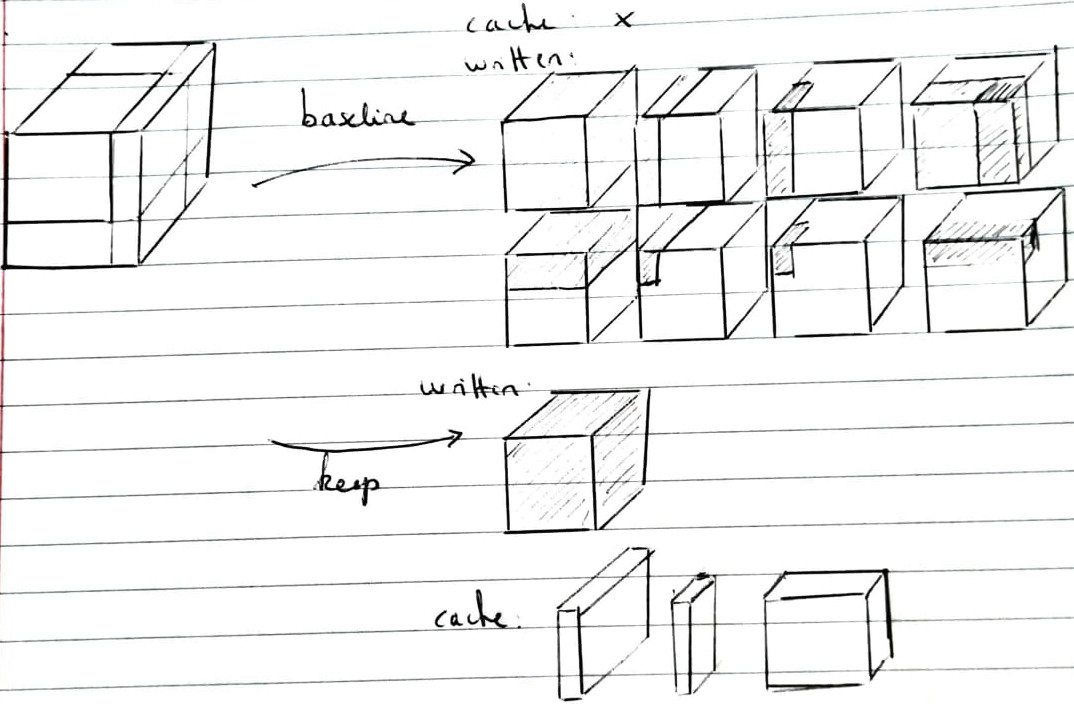
\includegraphics[scale=0.25]{./figures/new/naive_vs_keep.jpeg}
\caption{desc.}
\label{fig:keepvsbaseline}
\end{figure}

When loading a read buffer, we call \texttt{extra data} the data pieces that
are not contiguous in their output file(s) of destination.
The keep strategy tries to use read buffers of shape $B$ such that $B$ covers
at least one output file completely i.e. $B_x>O_x$ for all dimensions $x$.
Such a buffer shape would allow to always have extra data in case of a shape
mismatch, hence making the cache management possible to reduce the number of seeks.
Indeed, it would allow to store the extra data into the cache in order to write
an output file only when all its data has been loaded.
We call this ideal read buffer shape $\Lambda$.
If $m$ is too small, then the keep strategy will find a buffer
shape as closed as possible from $\Lambda$.

The implementation of the keep strategy for
Algorithm~\ref{algo:generalrepartition} consists in implementing
getReadBuffers and getWriteBuffers.

\subsection{Input aggregates}
getReadBuffers finds the buffer shape $B$ that is the closest to the optimal buffer
shape $\Lambda$, such that $\Lambda_x>O_x$ in any dimension $x$.
If $I_x > O_x$, then $\Lambda_x$ can be set to $I_x$. If $I_x < O_x$ however,
$Lambda_x$ must be a multiple of $I_x$ in order to keep reading each input
block part in one seek (for opening the file).
We define an \texttt{input aggregate} as being the minimum aggregate of input
files that covers one output file completely. In particular, $\Lambda$ is the
input aggregate that covers the first output file (indexed $(0,0,0)$) in the
original image being re-partitioned.

\subsection{Searching for the optimal buffer in the inverse storage order}

For the \texttt{C-order} and given the analysis of the baseline algorithm,
it seems better to have a buffer shape that stores extra data in the $k$
dimension first, rather than in the $j$ or $i$ dimension.
Therefore, if $m$ is too small to get $B=\Lambda$, one must try to get
$B_k=\Lambda_k$ first, then $B_j=\Lambda_j$ and $B_i=\Lambda_i$, i.e. in the
inverse of the storage order (the C-order: $i\rightarrow j\rightarrow k$).

In practice, the buffer is initialized as $B=(1,1,\Lambda_k)$ which means
that we can read one complete data column from an input block and keep the
remainder in memory for the next buffer.
Note that we assume that $m$ is large enough to store a buffer of shape
(1,1,$\Lambda_k$).
If it was not the case the keep algorithm would not give a significant
improvement in the number of seeks produced by the repartition task, compared
to the baseline algorithm.

\subsection{Bruteforce search of the read buffer shape}
We found that stretching the buffer step by step in the $j$ and then in the
$i$ dimension does not reduce $s$
in a strictly decreasing way which mean we may go over local minima.
We therefore decided to compute the quantity of seeks produced for all the
possible buffers together with their maximum RAM consumption.
It is then possible to find the buffer shape producing the less seeks, subject
to $m$.

There is not an infinite possibility for the buffer shapes;
Firstly, the only possibilities for the buffer dimensions are the integer
divisors of R, such that $B_i*B_j*B_k < m$. Indeed, the buffer dimensions must
be integers and the buffer shape B must be a partition of R.
Secondly, as it has been said in the previous subsection, we are only
interested in buffer shapes following the inverse storage order. It implies that
we are only interested in buffers that are of the form $(1,1,R_k)$,
$(1,B_j,R_k)$ or $(B_i,R_j,R_k)$.

\subsection{Impact of the buffer order on performance}
Using the keep strategy, one may order the buffer loadings to reduce the maximum
quantity of extra data stored in memory, hence, reducing the amount of seeks.
For example, if the shape mismatches occur only in the $k$ axis, loading the
buffers in this direction will enable recycling the extra data in cache,
resulting in a smallest memory consumption over time.
The memory saved thanks to a smart
ordering could enable the storage of more overlaps in memory using the
``keep strategy", further reducing the overall number of seeks.

As explained in the discussion, the buffer ordering problem is complex and does
not seem easily solvable.
This study uses a naive order which is, again, the inverse storage order.
Note that using such
an order allows recycling extra data in the $k$ dimension first, it is therefore
most efficient when the biggest overlap between input and output files is in the
$k$ dimension.

Thanksfully, the impact of the buffer ordering on performance can be
mitigated. Indeed, the impact of the buffer ordering depends on the size of the
mismatches. One can reduce the amount of extra data by using smallest chunks: Even
if the overlap between the input and output files is big with respect to their
size, the area/volume of the overlap will be kept small.

\subsection{Remainder volumes}

getWriteBuffers defines the blocks of data that will be written at once in each
output file.
To find these buffers, we first need to define what a remainder volume is.

A read buffer of shape $\Lambda$ can be divided in
8 parts or ``volumes" (Figure~\ref{fig:nomenclature_overlaps}).
7 out of these 8 volumes are called \texttt{remainder volumes} because
they are created by the shape mismatch between the input files and the output files on
the buffer borders.
The 7 remainder volumes enclose an 8th part that is composed of
input files that are either complete or which complementary part have already
been loaded by a previous buffer. This means that any complementary part is either
in memory (it has been kept in cache according to the keep strategy) or it has
been written down previously.
In other words the remainder volumes contain non contiguous parts of output blocks
as opposed to the non-remainder volume which contains a contiguous part of
an output block.
For each buffer, each of volume
is indexed following the buffer order $F_0$ to $F_7$, with $F_0$ being the
non-remainder volume. If the buffer is smallest than the input aggregate or if
there is no shape mismatch in a given dimension, it may be that a volume size
is set to 0.
Note that a single remainder volume can contain several output file parts.

\begin{figure*}[h]
\centering
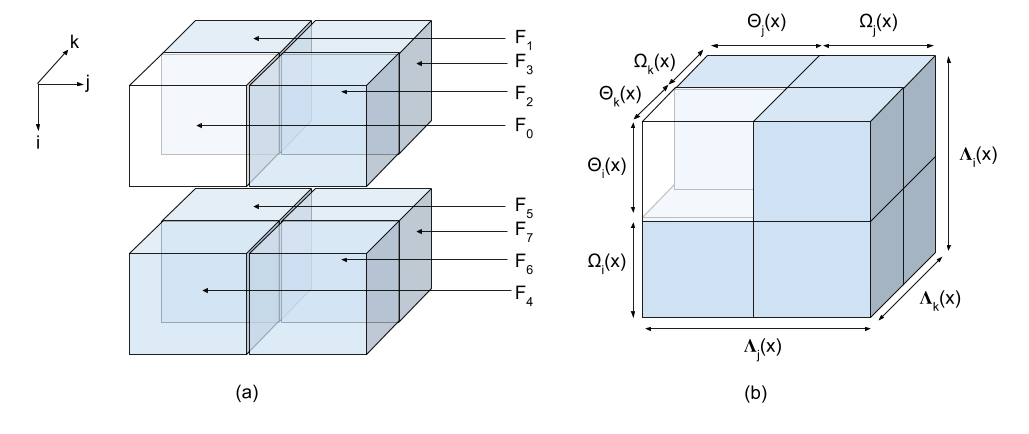
\includegraphics[scale=0.4]{./figures/new/nomenclature_overlaps.png}
\caption{Division of a buffer into 8 parts indexed according to the storage
order, 7 of which are remainder volumes.}
\label{fig:nomenclature_overlaps}
\end{figure*}

In the baseline algorithm, the write buffers are defined as the
intersection between the read buffers and the output blocks.
In the context of the keep strategy, some of the remainder volumes are kept
to be written together with other remainder volume(s) contiguously in the output
blocks.
This is equivalent to initializing the write buffers with the same definition as
in the baseline algorithm, and then fusing some of them to be written at once.
The way in which the remainder volumes are fused is summarized in
Table~\ref{tab:fusion}.

\begin{table}[ht]
  \centering
  \caption{Direction(s) in which to fuse the write buffers according to the keep strategy}

   \begin{tabular}[t]{c c }
   \hline
   remainder index & direction to fuse \\
     \hline\hline
     1 & k \\
     \hline
     2 & j \\
     \hline
     3 & j,k \\
     \hline
     4 & i \\
     \hline
     5 & i,k \\
     \hline
     6 & i,j \\
     \hline
     7 & i,j,k \\
     \hline
   \end{tabular}

   \label{tab:fusion}

\end{table}

\subsection{Maximum memory consumption}

In order to perform the bruteforce search of the best read buffer shape $B$,
we need a way to compute the maximum memory consumption of the algorithm using
this shape.
Having partitioned the buffers into volumes, the maximum memory consumption can
be computed by simulating the re-partition algorithm and computing, at each step,
the cache size.

Let us define $\Sigma$, the amount of data in RAM at a given time during the
execution of the re-partition algorithm.

In order to compute $\Sigma$, the volumes' sizes need to be computed using the
following nomenclature (Figure~\ref{fig:nomenclature_overlaps}):
Given a buffer shape $B$ and the output file shape $O$, we define $C_d(x)$ as
the overlap length between the buffer and an overlaping output file in direction
$d$ for the $x^{th}$ buffer. Let us define $\Omega$ and $\Theta$, that are used
to define upper bounds in the volumes sizes formulas. $\Omega_d(x)$ is the
equivalent of $C_d(x)$ if the buffer was of shape $\Lambda$, and $\Theta_k(x)$
is the difference between $B_d$ and $\Omega_b$, with $B=\Lambda$.
These metrics are computed as follows:
$$C_d(x) = (x+1)B_d mod(O_d)$$
$$\Omega_d(x) = (x+1)\Lambda_d mod(O_d)$$
$$\Theta_d(x) = \Lambda_d - \Omega_d(x)$$

\subsection{Seek estimation for the keep strategy}

In order to compute the amount of seeks produced by running the re-partition
algorithm using the keep strategy with a given read shape $B$, we computed this
amount as the sum of the amount of seeks caused by loading the read buffers $s_r$
and the amount of seeks caused by writing the write buffers $s_w$,
such that $s=s_r+s_w$.

When loading the read buffers, the seeks occur in case of a shape mismatch
between a read buffer and the input files. It is the exact same problem than
when computing the amount of seeks produced by the baseline algorithm when
writing in the output files. Therefore, the baseline seek model presented
before can be used to compute $s_r$.

In order to compute the amount of seeks produced by the write buffers however,
we did not find an elegant formula to solve the problem. We can compute $s_w$
by first finding the write buffers, and then summing the amount of seeks done
by each write buffer. Indeed, given a dimension $x$, a write buffer will seek
if its length in the $x^{th}$ dimension is different than $O_x$.

In particular, with $WB$ the write buffer shape,
\begin{itemize}
  \item $WB_k \neq O_k => WB_i*WB_j$ seeks.
  \item $WB_j \neq O_j => WB_i$ seeks.
  \item $WB_i \neq O_i => 1$ seeks.
\end{itemize}

%----------------------------------------
\section{Implementation}
%----------------------------------------



%----------------------------------------
\section{Experiments}
%----------------------------------------



\subsection{Experimental setting}
The experiments have been executed under the same conditions, on a private
cluster using \texttt{slurm} as workload manager. Each compute node has 256GB of
RAM, 6 SSDs of size 480 GB and 32 cores. We only used 1 node and 1 SSD at a
time. The Python environment used was a
conda environment, all packages used together with their version are available
in a \texttt{requirements.txt} file. The instructions about how to install the
dependencies in a virtual or
conda environement are provided in the \texttt{README} file of the
\href{https://github.com/GTimothee/repartition_experiments}{project's repository}. The
code for all experiments can be found in the same repository as well.

\subsection{Results}

%----------------------------------------
\section{Discussion}
%----------------------------------------

\subsection{The buffer ordering problem}
The buffer ordering problem can be modeled as follows: We can represent the
problem as a complete bidirectional graph in which each vertex is a buffer. At
initialization, we must choose a first buffer as an entry point. Let us define
a path in the graph as a visitation order of all buffers in the graph. One buffer
cannot appear twice in the list. Finally, let us define a cache that contains
the data currently in main memory. We define the buffer ordering problem as the
problem of finding the optimal path such that the amount of memory used by the
cache is kept minimal during the process. For each buffer, we load some data
into the cache (reading the buffer) and free some of it (writing into output files).
The amount of
data released is different depending of the buffers previously visited and each
buffer can only be visited once which can be represented by removing all edges
pointing to a visited vertex except the one coming from the previously visited
vertex. One may solve this problem by using a greedy algorithm or a shortest path
algorithm but it would
incur more infering at runtime and a potentially complex algorithm to run.
We decided to keep things simple using a naive buffer order, the storage order,
as the goal of this study was primarily to assess if the keep algorithm works.

\subsection{Breaking the buffers}
To even reduce the maximum amount of memory used during the repartition process, we
could read the input files one by one instead of enforcing \texttt{dask} to read a whole
buffer at a time, provided that the input files' parts are read in the right
order (following the buffer order). The idea of reading an entire buffer at a
time came from the clustered and multiple strategies but we realized afterwards
that this could be beneficial to break the buffers into input files' parts. We
can see in Equation (2) that it would result in replacing $B_iB_jB_k$ by
$I_iI_jI_k$ or less if part of a file is loaded. This idea would only be
beneficial in the case where $B_x>I_x$. Indeed, in the other case, the buffer is
loaded anyways.

\subsection{ROI extraction problem}
The Region Of Interest (ROI) extraction problem is a related problem that still needs
to be adressed. A solution using chunking as been introduced in~\cite{optimal_chuking}. The authors
define an array partitioned into chunks of equal shapes and then define a
query as an arbitrary subarray of the input, chunked, array. They define the
optimal chunking problem as finding the optimal chunk such that the expected
number of chunks retrieved to answer the query is minimal. In our opinion, the
solution in~\cite{optimal_chuking} is limited due to the need of historical or theoretical workload
and the necessity to repartition the input array into an ``optimal" chunk shape. We
would prefer letting the application choose the appropriate chunk shape
regarding its needs and not needing to estimate the processing workload. We
define the ROI extraction problem as follows: Finding an algorithm that takes
as input an arbitrary chunk shape and extract the ROI data from the chunks with
the less number of seeks as possible.

\subsection{Solving three problems at once}
As stated in the introduction, the split and merge tasks are special cases of
the repartition task. This observation leads us to think that maybe one could find
one optimal algorithm for the split, merge and repartition tasks.

If we were to use the keep algorithm with $I=R$, we would read the input data
in slices, exactly like the multiple strategy. The only difference between the
two strategies, however, is that if some remainders appear at the bottom of the
buffer, the keep algorithm would keep it to try to read and write files in one
seek. Not only the keep algorithm tries to limit seeking into the files but it
also tries to limit switching between the files. It would be interesting to
compare the two algorithms for the split/merge tasks to see if the keep
implementation brings any kind of improvement.

\subsection{Towards distributed systems}
A future work would be to find distributed versions of the split/merge/repartition
algorithms. Lots of scientists use HPC (High Performance Computing) clusters
regularly which brings considerations about how to use such distributed
algorithms with Lustre for example, a commonly used filesystem for HPC. \texttt{dask}
also provides a distributed scheduler that seems to be quite efficient. It is
now recommended for use, even on local computers (using one node).

%----------------------------------------
\section{Conclusion}
%----------------------------------------

%----------------------------------------
\section{Acknowledgments}
%----------------------------------------

\bibliography{Bibliography}
\bibliographystyle{ieeetr}

\end{document}
